\documentclass[../main.tex]{subfiles}
\graphicspath{{\subfix{../diagrams/}}}
\begin{document}

State diagrams show states of orders (both shop and client module), shop employee, courier
and complaints. The other objects did not require such a detailed description of their states due to their obvious action.

\subsection{Order (shop module)}
\vspace{5mm}
\makebox[\textwidth]{\includegraphics[width=0.75\textwidth]
{diagrams/states-diagrams/states_Zamowienie-sklep.pdf}}

Object Order in shop module has a field \textit{OrderState} which can take following values:

\begin{itemize}
\item WaitingForCollection,
\item Collecting,
\item WaitingForCourier,
\item ParcelCollected,
\item OnTheWay,
\item Delivered
\end{itemize}

\vspace{5mm}
Diagram illustrates how the shop can see an manage the order. It is divided into two parts, first represents states connected with the shop while the second one states connected with courier. First of all orders are made by client and before that time shop doesn't have access to it. Once the order is submitted by a client it gains status as \textbf{WaitingForCollection} . It means that the order is already in system and it waits for a shop worker to start collecting it. There is a need for that state because it is a start state and a worker may be busy collecting other orders. There can be a lot of orders in that state in the same time. 

Worker starts collecting the order and changes it status to  \textbf{Collecting}. Now he can see products and their amount he needs to find and collect. After the worker submits completing the order it changes its status to \textbf{Waiting for courier}. The order is packed and is waiting for a courier to take it and after that action it changes its state to \textbf{Parcel collected}.

In the part connected with courier when courier has parcel is going straightly to the client it changes state to \textbf{On the way}. There is a difference between this and previous state because \textbf{Parcel collected} means that parcel left the shop but courier can have many parcels so he can go to another client earlier. As soon as courier arrives to client and give him the parcel the state changes to \textbf{Delivered} and that is the end state.

\subsection{Order (client module)}
\vspace{5mm}
\makebox[\textwidth][c]{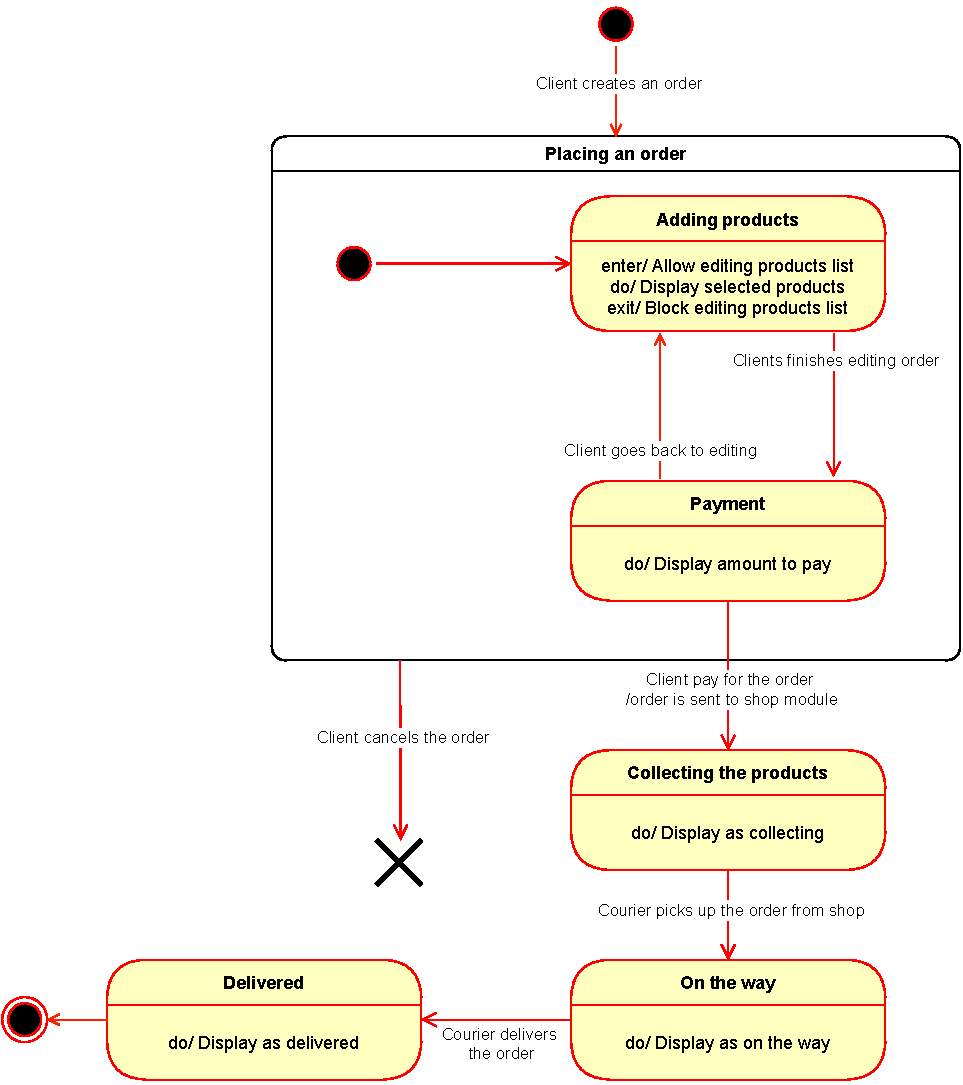
\includegraphics[width=0.75\textwidth]
{diagrams/states-diagrams/states_Zamowienie-klient.pdf}}

Object Order in client module has a field \textit{CurrentState} which can take following values:

\begin{itemize}
\item AddingProducts,
\item Payment,
\item CollectingProducts,
\item OnTheWay,
\item Delivered
\end{itemize}
\vspace{5mm}
Diagram illustrates how the shop can see an manage the order. It is divided into two parts, first represents states connected with the placing an order while the second one states connected with courier.In the first part when client decides to make an order then it comes to starting state \textbf{AddingProducts}. Client can see list of products, can add products to the list and also delete products from the list. When he decides that he has chosen all products he go to the payment section and state changes to \textbf{Payment}. Payment section display amount of money to pay and display available payment methods. Client can still go back to editing the order which makes again \textbf{AddingProducts} state. Client can also cancel the order which result in deleting the Order object.

Once a client accepts the order, it is sent to the shop module and the state changes to \textbf{CollectingProducts}. It means that shop got notification about the order and the realization is in progress. When the collection of products is completed and courier is straightly on the way to client the order changes its state to \textbf{On the way}. When the courier arrives at right address and delivers the order it changes status to \textbf{Delivered}.

\subsection{Shop worker}
\vspace{5mm}
\makebox[\textwidth][c]{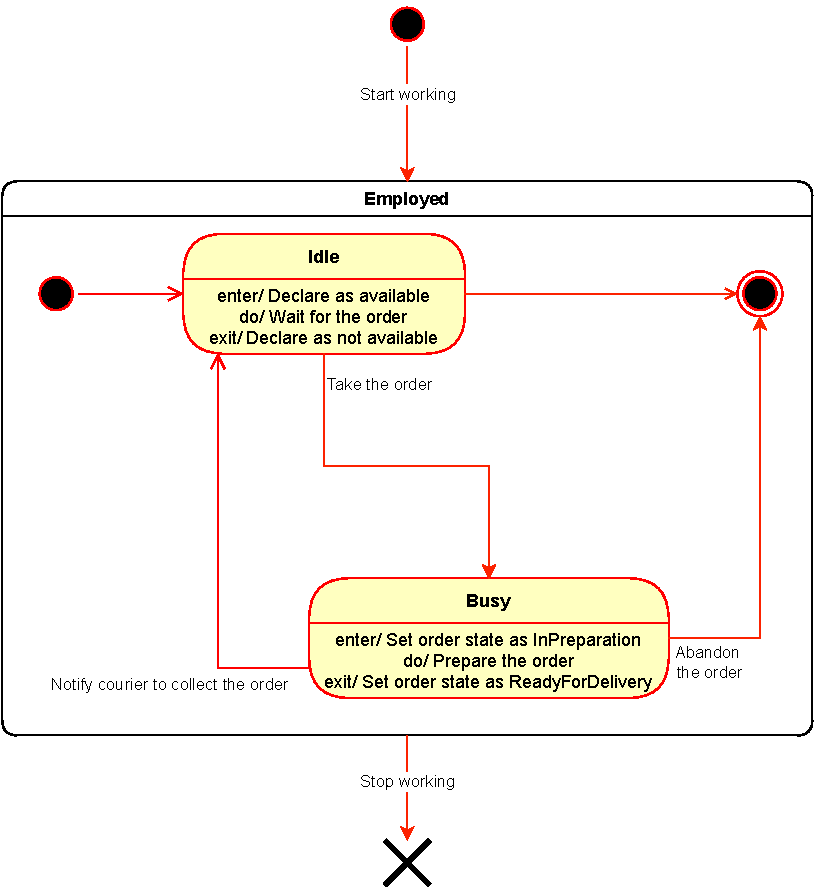
\includegraphics[width=0.75\textwidth]
{diagrams/states-diagrams/states_Pracownik sklepu.pdf}}

Object ShopEmployee in shop module has a field \textit{CurrentState} which can take following values:

\begin{itemize}
\item Idle,
\item Busy
\end{itemize}

Shop worker has two states. He can be in \textbf{Idle} state which means he is declared as available and waits for the orders. Then he changes status to \textbf{Busy} which means he is in progress of completing the order.


\subsection{Courier}
\vspace{5mm}
\makebox[\textwidth][c]{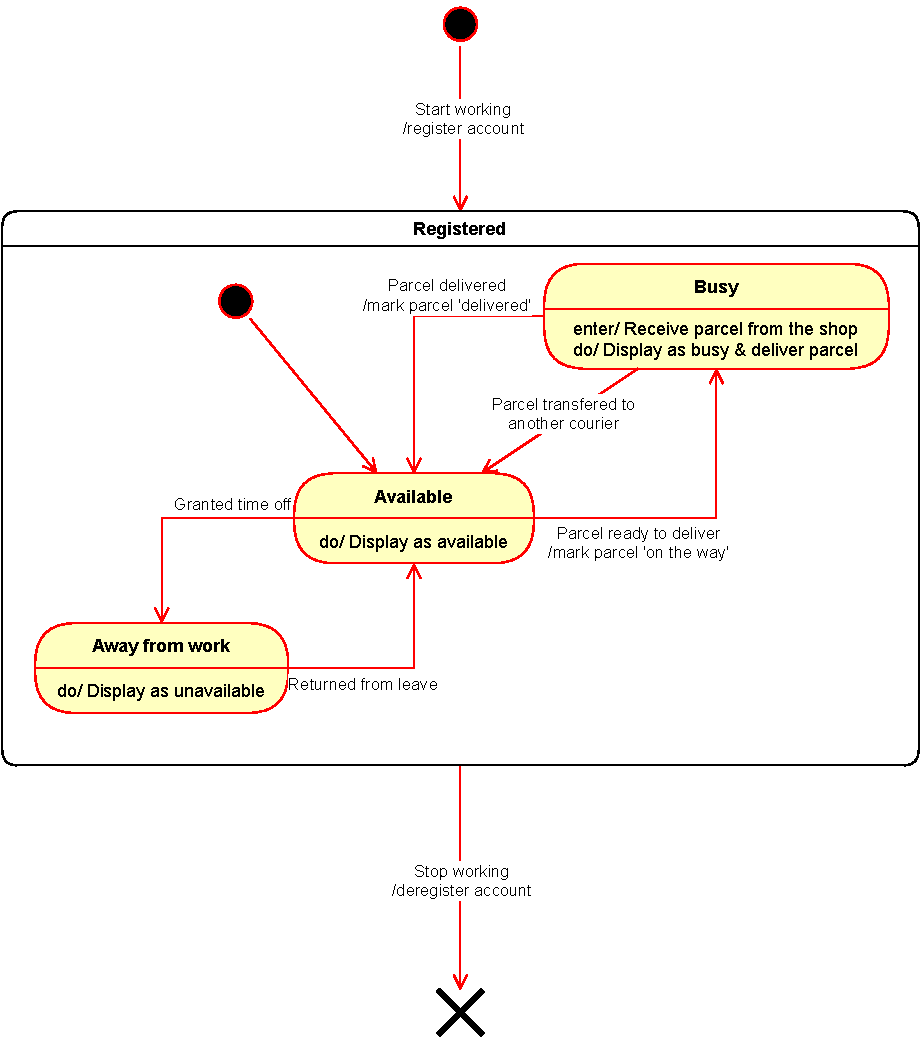
\includegraphics[width=0.75\textwidth]
{diagrams/states-diagrams/states_Kurier.pdf}}

Object Courier in Delivery module has a field \textit{CurrentState} which can take following values:

\begin{itemize}
\item Available,
\item Busy
\item AwayFromWork
\end{itemize}
\vspace{5mm}
The object of Courier is created when someone register his account. The staring state is \textbf{Available}. In this state a courier is available to work he is waiting for orders from the shop. Courier can log out or have a break which means that he the state of him changes to \textbf{AwayFromWork}. In this state courier can log in or come back from break which result in coming back to \textbf{Available} state. When courier is on the way to shop or on the way to client he changes his status to \textbf{Busy}. After delivery of package to the client it changes status to \textbf{Available}.

\subsection{Complaint}
\vspace{5mm}
\makebox[\textwidth][c]{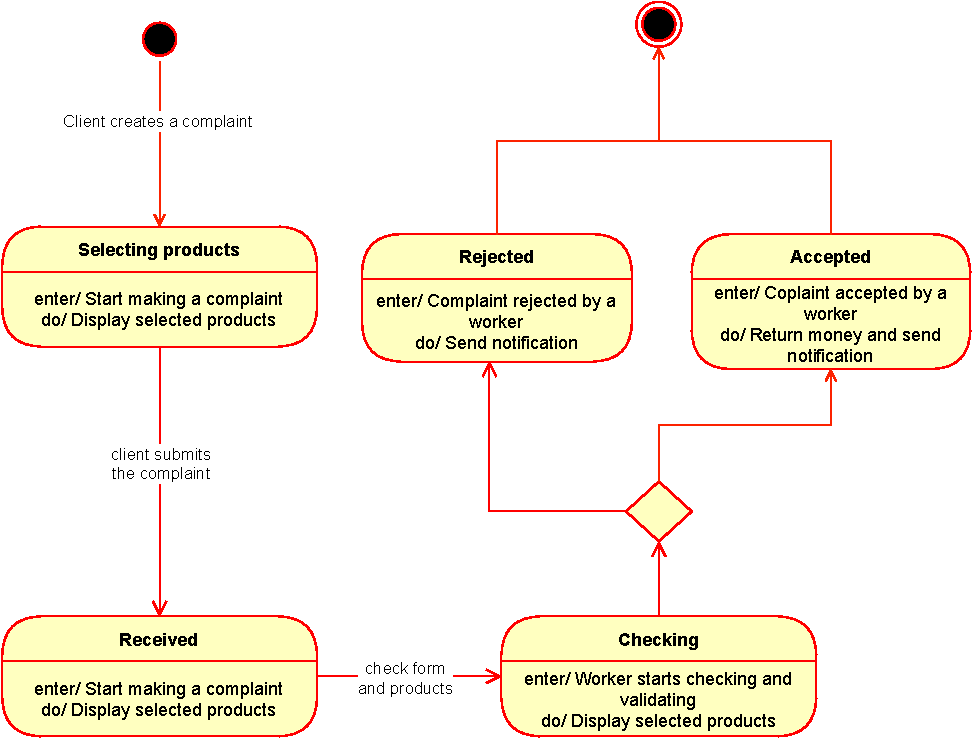
\includegraphics[width=\textwidth]
{diagrams/states-diagrams/states_Reklamacje.pdf}}

Object Complaint in Client module has a field \textit{CurrentState} which can take following values:

\begin{itemize}
\item SelectingProducts,
\item Received,
\item Checking,
\item Accepted,
\item Rejected
\end{itemize}

Client can create a complaint to complain products which did not meet the client's expectations. Starting state is \textbf{SelectingProducts}. Client has form presenting products with option to select which of them he wants to complain. After the client submit the complaint the notification is send to the shop. When the shop receives the complaint changes state to \textbf{Received} and awaits for shop worker to check if the complaint is right and justified. When shop worker is checking the complaint it gets status \textbf{Checking}. Worker can see selected products and accept or reject the complaint. If the complaint is rejected the state of complaint changes to \textbf{Rejected} and notification to client is send. If the complaint is accepted the state of complaint changes to \textbf{Accepted} and notification to client is send. 

\end{document}